  % ------------------------------------------------------------------------------
  \section{Applications}
  \label{sec:applications}
  % ------------------------------------------------------------------------------

  In this section, we present a number of applications involving path traversal
  in triangulations.
  These applications employ the data structures described in Sections \ref{sec:tins}
  and \ref{sec:point_location}.
  The applications, in particular those described in 
  Section~\ref{ssec:ter_profile_tpath}, deal with triangulations used to model 
  terrains.
  A terrain model is a digital model of some surface.
  Most often the surface being modeled is some region of the earth, but any surface
  with relief can be modeled.
  Triangulations, commonly refered to as Triangular Irregular Networks, or TINs 
  in this context, are one means of modeling a digital terrain.
  In a TIN, the point set $\pointset$ is a set of points of known elevation. 
  Given a triangulation, $\triang$, built on $\pointset$, the elevation for any
  point, say $q$, on the surface can be readily estimated from the vertices
  of the triangle containing $q$.
  In addition to $x$ and $y$ coordinates, each point in $\pointset$ stores a $z$
  coordinate which records the elevation.
  Such models are sometimes refered to as 2.5 dimensional, since they cannot 
  properly represent a truly three-dimensional surface (for example there is no
  way for a planar triangulation to represent an overhanging cliff). 

  We begin by describing two simple and closely related queries, 
  reporting terrain profiles, and trickle paths, in 
  Section~\ref{ssec:ter_profile_tpath}.  
  In Section~\ref{sec:con_comp_queries}, we present a slightly more complex 
  application of our data structures, 
  reporting connected components of a triangulation (or terrain). 
  We start with the simpler case of reporting a component which is a convex
  subregion of the triangulation, and then describe methods for the more 
  general case where the connected component may represent a non-convex region.
  As all the queries we describe in this section require that a starting 
  triangle in the mesh be identified, we will assume that this triangle
  is given as part of the query.
  In practice, most of the queries we describe here can use a start triangle,
  identified by answering a
  single planar point location query using the technique outlined in 
  Section~\ref{sec:point_location}.

  \subsection{Terrain Profiles and Trickle Paths}\label{ssec:ter_profile_tpath}

  Terrain profiles are a common tool in GIS visualization. 
  The input is a line segment, or chain of line segments possibly forming a polygon, 
  and the output is a profile of the elevation along the line segment(s). 
  The trickle path, or path of steepest descent, from a point $p$ is the path on
  the terrain, represented by $\triang$, 
  that begins at $p$ and follows the direction of steepest descent until it reaches 
  a local minimum or the boundary of $\triang$ \cite{DBLP:conf/cccg/BergBDKOGRSY96}. 
  Both queries involve traversing a path over $\triang$, with the fundamental 
  difference being that in the terrain profile the path is given, whereas in 
  reporting the trickle path, the path is unknown beforehand and must be 
  determined based on local terrain characteristics.

  In analyzing these algorithms, we measure the complexity of a path by length 
  of the sequence of triangles visited, which we denote by $K$. 
  When a path intersects a vertex, we consider all triangles adjacent to that 
  vertex to have been visited. 
  Given this definition, we have the following result for terrain profile and 
  trickle path queries:

  \begin{lemma}\label{lem:tprofile_tpath}
  Let $\triang$ be a terrain stored using the representation described
  in Theorem~\ref{thm:terrain_traversal}, then:
  \begin{enumerate}[label={(\alph{*})}]
  \item{ Given a chain of line segments, $S$, the profile of the intersection 
  of $S$ with $\triang$ can be reported with $\BigOh{ \frac{K}{\lg{B}} }$ I/Os.}
  \item{ Given a point $p$ the trickle path from $p$ can be reported with 
  $\BigOh{ \frac{K}{\lg{B}} }$ I/Os.}
  \end{enumerate}
  \end{lemma}

  \begin{proof}
  Let $S$ be a chain of $i$ segments, denoted $s_0, s_1, \ldots s_i$. 
  In order to report an elevation profile, start at the endpoint of $s_0$, and 
  let $t \in \triang$ be the triangle which contains this endpoint. 
  We calculate the intersection of $s_0$ with the boundary of $t$ in order to determine 
  which triangle to visit next. 
  If at any point in reporting the query the next endpoint of the current segment 
  $s_j$ falls within the current triangle, we advance to the next segment 
  $s_{j+1}$. 
  This procedure is repeated until the closing endpoint of $s_i$ is reached.
  This query requires walking a path through $T$ that visits exactly $K$ triangles.

  For the trickle path, we are given triangle $t$ and some point interior to $t$. 
  The trickle path from $p$, and its intersection with the boundary of $t$, 
  can be calculated from the coordinates of the point vertices adjacent to $t$. 
  If the path crosses only the faces of triangles, we can simply report the 
  intersection of the path with those triangles.
  By Theorem \ref{thm:terrain_traversal}, it 
  requires $O(K/\lg{B})$ I/Os to report a path crossing $K$ triangles. 
  When an edge is followed, visiting both faces adjacent to that edge no more 
  than doubles the number of triangles visited. 
  The only possible problem occurs when the path intersects a point vertex. 
  Such cases require a walk around the point vertex to determine through which 
  triangle 
  (or edge) the path exits, or if the point vertex is a local minima. 
  In this case, the path must visit each triangle adjacent to the point vertex 
  through which it passes, thus all triangles visited during the cycle around a 
  point vertex are accounted for in the path length $K$.
  \end{proof}

  % -------------------------------------------------------------------------
  \subsection{Connected Component Queries}\label{sec:con_comp_queries}
  % -------------------------------------------------------------------------

  In this section, we describe how connected component queries can be reported 
  using our data structures. 
  We begin by defining \emph{connected component} and \emph{connected
  component query} in this setting.
  Let $\triang$ be a triangulation, and let $t$ be a triangle in $\triang$. 
  We denote by $\mathcal{P}(t)$ some property that is true for $t$.
  This property may be some value stored for each triangle, or some value that
  can be computed locally, such as slope or aspect if $\triang$ is a terrain.
  The connected component of $t$ with respect to $\mathcal{P}$ is the 
  subset $\concomp \subset \triang$, such that following conditions hold for
  all $t_c \in \concomp$:

  \begin{enumerate}
    \item $\mathcal{P}(t_c)$ is true, and
    \item there exists a path $t_1, t_2, \ldots t_n$ where $t = t_1$ and 
    $t_c = t_n$ such that $\mathcal{P}(t_i)$ is true for all $i$, and $t_i$ 
    and $t_{i+1}$ are adjacent.
  \end{enumerate}

  In order to simplify the discussion that follows, we adopt two conventions that we use
  throughout this section. 
  Firstly, while we assume that $\triang$ is represented by its augmented dual
  graph $\augdual{\triang}$, we will describe the various algorithms in terms
  of operations on the dual graph $\dual{\triang}$. 
  Furthermore, when we can do so without confusion, we use a single identifier
  to represent both a triangle and its corresponding node in the dual.
  For example, if we have triangle $t \in \triang$ corresponding to  
  $\dual{t} \in \dual{\triang}$, we may use $t$ in reference to both the
  triangle and the dual node.

  The second convention we will adopt relates to $\mathcal{P}$.
  If $\mathcal{P}(t)$ is true, then we call $t$ a \emph{red} node (triangle).  
  If $\mathcal{P}(t)$ is false, then we call $t$ a \emph{black} node (triangle).

  In Section~\ref{ssec:conv_con_comp} we address queries 
  where the component being reported is convex. 
  This constraint is not as limiting as it may seem.
  For example, rectangular window queries, a very common type of query, 
  may be viewed as a specialized case of reporting a convex 
  component.
  In Section~\ref{ssec:gen_con_comp}, we deal with the more challenging 
  problem of reporting
  connected components where the component may be non-convex.

  % -------------------------------------------------------------------------
  \subsubsection{Convex Connected Components}\label{ssec:conv_con_comp}
  % -------------------------------------------------------------------------

  Before describing the reporting of convex connected components, we show how 
  to solve a related problem. 
  Given the dual of a convex triangulation, $\dual{\triang}$, and a 
  vertex $\dual{s} \in \dual{\triang}$, 
  perform a depth-first traversal of $\dual{\triang}$, starting at $s$, without 
  using mark bits.
  Mark bits are commonly used in depth-first traversal to record which vertices 
  have already been visited. 
  However, their use is infeasible with our data structures, due to the 
  duplication of the vertices of $\dual{\triang}$.
  Mark bits would require that we find and mark all duplicates of 
  a vertex whenever it is visited.
  This entirely defeats the purpose of our data structure.

  In order to avoid the use of mark bits, we select from among the edges incident 
  to each node a single \emph{entry} edge for that node. 
  While performing a depth-first traversal, we extend the traversal 
  to a node only along its entry edge.
  This leaves us with the problem of determining how to select the entry edge
  for a node.  
  Gold and Maydell~\cite{gold_maydell_1978} and Gold and 
  Cormack~\cite{gold_cormack86} demonstrated how such an entry edge could 
  be selected to enable depth-first traversal on a triangulation.
  Their approach identified one of the three edges of a triangle as its 
  entry edge.
  Since there is a one-to-one correspondence between the edges in $\triang$ 
  and $\dual{\triang}$, we can apply such a rule to identifying entry
  edges for nodes in $\dual{\triang}$. 
  De~Berg~\etal~\cite{deberg_et_al_1997} showed that the same technique can 
  be applied to the more general case of planar subdivisions, and 
  gave an entry-edge selection rule for polygons that, naturally, also works 
  for triangles.
  De~Berg's selection rule operates as follows\footnote{We 
  omit some minor details that are not relevant to triangles.}:

  \begin{enumerate}
  \item Let $t_s$ be a triangle in $\triang$, and let $s$ be a point interior
  to $t_s$.
  \item Let $t$ be the triangle for which we wish to identify an entry edge.
  Calculate the distance from $s$ to the closures of all edges of $t$.
  Let $s'$ be the point on $t$ that minimizes $\texttt{dist}(s,s')$. 
  \item If $s'$ is interior to an edge of $t$; select this edge as the
  entry edge, otherwise, $s'$ must be a vertex of $t$. 
  In this case, let $e$ and $e'$ be the edges adjacent to $s'$. 
  If $e$ is \emph{exposed} to $s$, such that the line $\vec{\ell}$ induced by 
  $e$ has $s$ strictly to its right, then select $e$ as the entry edge, otherwise
  select $e'$. 
  \end{enumerate}

  Now consider the graph $\dual{\triang}$.
  If we remove all edges from $\dual{\triang}$ that
  do not correspond to entry edges in $\triang$, we are left with a tree, 
  rooted at $t_s$ (see Figure \ref{fig:imp_tree_entry}).
  Proof of this claim can be found in~\cite{deberg_et_al_1997}.
  The triangle $t_s$, which contains $s$, has no entry edges itself.

  \begin{figure}[th]
	  \centering
		  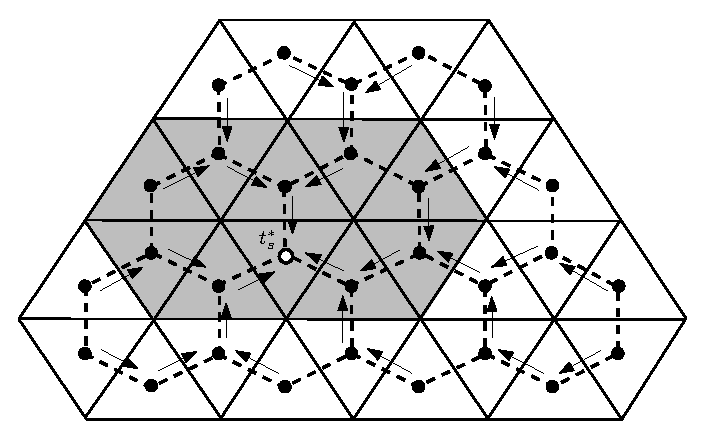
\includegraphics[width=0.6\textwidth]{Fig7}
	  \caption[Dual graph with non-entry edges removed forms a tree]{ 
	    A triangulation is shown with its dual graph. 
	    The blue arrows indicate the entry edges selected for each triangle when
	    triangle $t_s$ is selected as the root ($\dual{t}_s$ is circled). 
	    The arrows are directed from child to parent.
	    Removing the non-entry edges results in a tree in the dual, rooted at 
	    $\dual{t}_s$.
	    So long as a connected component is convex (e.g., the shaded area) this 
	    tree property holds for the subgraph consisting of only nodes in the
	    component.} \label{fig:imp_tree_entry}
  \end{figure}
	  
  \begin{figure}[th]
	  \centering 
	  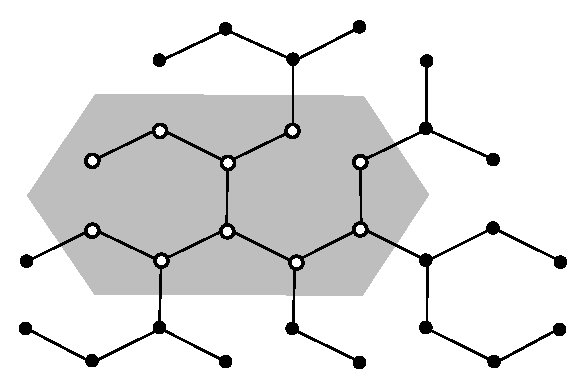
\includegraphics[width=0.6\textwidth]{Fig8}
	  \caption[Tree rooted at $t_s$]{ The tree rooted at $t_s$. 
	    The red nodes indicate nodes of the subtree contained within the 
	    connected component; this subtree is still connected even when all 
	    (black) nodes - which are not part of the component - 
	    are removed.} \label{fig:implicit_tree}
  \end{figure}

  This result leads to a simple traversal algorithm for connected 
  components, in the case where we know that the region to be reported 
  is convex.
  We summarize with the following lemma.

  \begin{lemma}\label{lem:report_convex_component}
  Let $\triang_C \subset \triang$ be a connected, convex component.
  Given $t_s \in \triang_C$ we can report all triangles in $\triang_C$ with 
  $\BigOh{\frac{|\triang_C|}{\lg{B}}}$ I/Os.
  \end{lemma}

  \begin{proof}
  Performing a depth-first search on a tree on $|\triang_C|$ vertices is equivalent 
  to walking a path of length at most $4 \cdot |\triang_C|$.
  By Theorem \ref{thm:terrain_traversal}, our data structures permit a walk along 
  such a path with a total I/O cost of $\BigOh{ \frac{|\triang_C|}{\lg{B}} }$.

  Let $s$ be some point interior to $\triang_C$, and let $t_s \in \triang_C$ be
  the triangle containing $s$.
  Starting with $t_s$, we implicitly construct a tree in $\dual{\triang}$ using the 
  selection method of~\cite{deberg_et_al_1997}.
  Since $\triang_C$ is convex, removing all subtrees rooted at black nodes results 
  in an implicit tree, rooted at $t_s$, which includes all red nodes in $\triang_C$
  (see Figures \ref{fig:imp_tree_entry} and \ref{fig:implicit_tree}).
  It remains to be proven that the removal of all subtrees rooted at black nodes
  will not result in the removal of any red nodes from the tree.
  Assume that removing the subtree rooted at some black node, $b$ removes some
  red node $r$. 
  Let $q$ be the parent of $b$ in $\triang_C$. 
  The entry edge corresponding to dual edge $(q,b)$ must be on the convex
  hull of $\triang_C$.
  However, this means that $r$ must be outside the convex hull of $\triang_C$, which
  is a contradition. 
  Therefore, no such triangle (node) $r$ can be removed.
  \end{proof}
  
  We give the following corollary to Lemma \ref{lem:report_convex_component}
  with application to rectangular window queries.
  Such queries are a specialization of reporting a convex region 
  and occur commonly in practice.

  \begin{corollary}\label{cor:window_query}
  Given a terrain $\triang$, and a query window $W$, the set of 
  triangles which intersect the query window can be 
  reported with $O \left( \frac{|\triang_W|}{\lg{B}} \right)$ I/Os. 
  \end{corollary}

  \begin{proof}
  The query window problem is equivalent to reporting 
  a connected component where the selection property is that a triangle 
  intersects the query window $W$. 
  The region to be reported is convex, but care must be taken with 
  triangles that intersect the query window boundary. 
  In \cite{deberg_et_al_1997} it is shown that the entry edge selection 
  rule can be modified to disqualify any edge (or portion thereof) that 
  is outside $W$. 
  Using this modification, an implicit rooted tree is still formed on 
  the triangles of $\triang_W$, and we can perform a memoryless 
  depth-first traversal.
  \end{proof}

  % --------------------------------------------------------------------
  \subsubsection{General Connected Components}\label{ssec:gen_con_comp}
  % --------------------------------------------------------------------

  In this section, we present an algorithm that reports connected components 
  that may be non-convex and/or contain holes.
  Using the terminology developed in Section~\ref{ssec:conv_con_comp}, we 
  say $\concomp$ is a connected component in $\triang$, corresponding 
  to $\dual{\concomp}$ in $\dual{\triang}$. 
  Recall that $\dual{\concomp}$ forms a connected component of red nodes 
  in the subgraph formed by all red nodes in $\dual{\triang}$.
  In $\triang$, we can think of the boundary of a connected component being 
  formed by all edges along the outer perimeter of the component
  in addition to any edges along the perimeters of holes. 
  In the dual, the boundary corresponds to the set of edges connecting 
  red vertices in $\dual{\concomp}$, with black vertices in $\dual{\triang}$. 

  In order to report $\concomp$, we select some triangle $s \in \concomp$ as our
  start triangle. 
  We select entry edges relative to an arbitrary point interior to $s$.
  Since $\triang$ itself is convex, we can construct an implicit tree
  on the nodes of $\dual{\triang}$, rooted at $s$.
  We denote this tree $\dual{\triang}_T$.
  
  Let $r$ and $b$ be red and black vertices in
  $\dual{\concomp}$, corresponding to adjacent triangles in $\triang$.
  Let $e$ be the edge of $\triang$ separating triangles $r$ and $b$.
  In $\dual{\triang}$, $e$ corresponds to the edge $(r,b)$.
  While this edge is undirected in $\dual{\triang}$, for the sake of the
  discussion that follows we will assume that in $\dual{\triang}_T$, it
  is directed towards the root, $s$.
  We call such edges \emph{boundary} edges, and classify them according
  to their role in the implicit tree $\dual{\triang}_T$, as follows 
  (see Fig.\ref{fig:imp_tree_non-convex}):
  
  \begin{enumerate}
    \item if $(r,b) \notin \dual{\triang}_T$, then $e$ is a \emph{wall}\footnote{
    All edges on the convex hull of $\triang$ are considered wall edges.} edge, 
    \item if $r$ is the parent of $b$, then $e$ is an \emph{access} edge, and 
    \item if $b$ is the parent of $r$, then $e$ is an \emph{exit} edge.
  \end{enumerate}

  \begin{figure}[th]
	  \centering
		  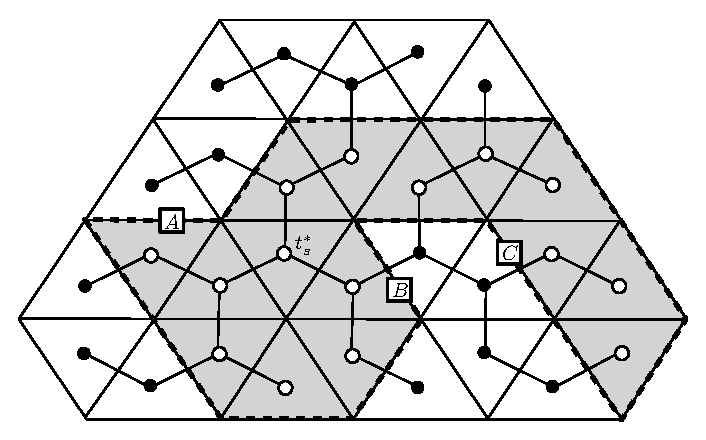
\includegraphics[width=0.6\textwidth]{Fig9}
	  \caption[Boundary edge definitions]{A triangulation and the implicit tree 
	  formed by the entry edges selected for the circled vertex $\dual{t}_s$. 
	  In this case, the connected component of $t_s$ is non-convex so that the tree 
	  formed by only red nodes is disconnected. 
	  The boundary edges of the triangulation are indicated by the heavy dashed 
	  blue line. 
	  Using our notation for boundary edges, A is a \emph{wall} edge, B is an 
	  \emph{access} edge where the tree enters the component, and C is an 
	  \emph{exit} edge where the tree leaves the component. }
	  \label{fig:imp_tree_non-convex}
  \end{figure}

  We report the triangles in $\concomp$ using the algorithm 
  $\funccase{DepthFirstTraversal}$ listed in Fig. \ref{fig:traverse_graph_algorithm}.
  $\funccase{DepthFirstTraversal}$ performs a standard depth-first traversal in 
  $\dual{\triang}_T$, with one important modification. 
  If a branch of the algorithm's execution terminates at an access boundary 
  edge, then the function $\funccase{ScanBoundary}$ (Fig. \ref{fig:scanhandrail_alg}) 
  is invoked. 
  $\funccase{ScanBoundary}$ traverses the chain of boundary edges, and recursively calls 
  $\funccase{DepthFirstSearch}$ at each exit edge. 
  A search structure, $\mathcal{V}$, is maintained to ensure that no boundary edge is 
  scanned more than once.  
  Whenever an access edge is visited during the $\funccase{ScanBoundary}$ 
  or $\funccase{DepthFirstSearch}$ 
  processes, it is added to the search structure $\mathcal{V}$ if it is not already 
  present. 
  If an access edge is encountered that is already in $\mathcal{V}$, then execution 
  of $\funccase{ScanBoundary}$ is halted. 
  Likewise, when $\funccase{DepthFirstTraversal}$ encounters an access edge already in 
  $\mathcal{V}$, it does not invoke $\funccase{ScanBoundary}$. 
  Figure \ref{fig:cmp_with_holes} demonstrates the operation of
  $\funccase{DepthFirstSearch}$ and $\funccase{ScanBoundary}$.

  \begin{figure}[h]
  \protect \framebox[0.95\linewidth]
  {
  \begin{minipage}{0.90\linewidth}

  \textbf{Algorithm $\textsc{\funccase{DepthFirstTraversal}}(t_s,s)$} \\
  1. \hspace{3pt} $t \leftarrow t_s$ \\
  2. \hspace{3pt} \textbf{do} \\
  3. \hspace{18pt} \textbf{if}($t$ has unvisited children) \\
  4. \hspace{33pt} $c \leftarrow $ next unvisited child of $t$ \\
  5. \hspace{33pt} \textbf{if}($\mathcal{P}(c) \ne \mathcal{P}(t)$) \\
  6. \hspace{48pt} $e \leftarrow$ boundary edge corresponding to $(c,t)$ \\
  7. \hspace{48pt} \textbf{if}($e$ is an access edge \textbf{and} $e \notin \mathcal{V}$) \\
  8. \hspace{63pt} $\funccase{ScanBoundary(e, t)}$ \\
  9. \hspace{48pt} \textbf{endif} \\
  10. \hspace{30pt} \textbf{else} \\
  11. \hspace{45pt} $t \leftarrow c$ \\
  12. \hspace{30pt} \textbf{endif} \\
  13. \hspace{15pt} \textbf{else} \\
  14. \hspace{30pt} $t \leftarrow$ parent of $t$ \\
  15. \hspace{15pt} \textbf{endif} \\
  16. \textbf{until}($t$ has no more unvisited children \textbf{and} $t=t_s$) \\
  \end{minipage}
  }
  \caption{Algorithm $\funccase{DepthFirstTraversal}$. }
  \label{fig:traverse_graph_algorithm}
  \end{figure}

  \begin{figure}[h]
  \protect \framebox[0.95\linewidth]
  {
  \begin{minipage}{0.90\linewidth}

  \textbf{Algorithm $\textsc{\funccase{ScanBoundary}}(e,t,s)$} \\
  1. \hspace{3pt} $e' \leftarrow$ next boundary edge in counterclockwise direction from $e$ \\
  2. \hspace{3pt} \textbf{do} \\
  3. \hspace{18pt} \textbf{if}($e'$ is an access edge) \\
  4. \hspace{33pt} \textbf{if}($e' \in \mathcal{V}$) \\
  5. \hspace{48pt} \textbf{break} \\
  6. \hspace{33pt} \textbf{else} \\
  7. \hspace{48pt} add $e'$ to $\mathcal{V}$ \\
  8. \hspace{33pt} \textbf{endif} \\
  9. \hspace{18pt} \textbf{endif} \\
  10. \hspace{15pt} \textbf{if}($e'$ is an exit edge) \\
  11. \hspace{30pt} select triangle $t$ adjacent to $e'$ \\
  12. \hspace{30pt} $\funccase{DepthFirstTraversal(t,s)}$ \\
  13. \hspace{15pt} \textbf{endif} \\
  14. \textbf{until}(e' == e) \\
  \end{minipage}
  }
  \caption{Algorithm $\funccase{ScanBoundary}$. }
  \label{fig:scanhandrail_alg}
  \end{figure}

  \begin{figure}[th]
	  \centering
		  \includegraphics[width=0.8\textwidth]{Fig10}
	  \caption[Traversal example on non-convex region with holes]{On the left is shown a 
	  triangulation $\triang$ and connected component $\triang_C$ (shaded) 
	  with a non-convex boundary and holes. 
	  The original tree $G_T$ is shown on the right, with vertices labeled by preorder 
	  number for the entire triangulation $\triang$. 
	  Hallow vertices correspond to vertices removed from $G_T$ by holes and/or 
	  concavities in the boundary of $\triang_C$. 
	  The parent-child relationships, as well as the vertex labels are also shown on $\triang$. 
	  In $\triang$ boundary edges are thick lines, with entry edges being dashed 
	  and exit edges dotted. 
	  The original call to $\funccase{DepthFirstTraversal}$ first encounters the 
	  entry edge 
	  (8,7), from which $\funccase{ScanBoundary}$ will visit exit edges (9,8), 
	  (12,11), and 
	  (14,13), in that order, before terminating back at $(8,7)$. 
	  This initial call to $\funccase{ScanBoundary}$ results in subtrees rooted
	  at vertices 
	  $9$, $12$, and $14$ being reported. 
	  $\funccase{ScanBoundary}$ is not invoked from entry edge (10,2), as this 
	  edge is added 
	  to $\mathcal{V}$ during the invocation of $\funccase{ScanBoundary}$ from 
	  $(8,7)$. 
	  $\funccase{ScanBoundary}$ is, however, called from $(17,1)$, which results 
	  in entry 
	  edges $(26,18)$, $(24,19)$, and $(20,19)$ being visited and the subtrees 
	  rooted at vertices $26$, $24$, and $20$ being reported.
	  The dashed arrows represent cases where $\funccase{ScanBoundary}$ jumps 
	  between
	  \emph{access} edges and \emph{exit} edges.}
	  \label{fig:cmp_with_holes}
  \end{figure}

  \begin{lemma}\label{lem:cc_holes_alg_correctness}
  Given a triangle $t_s \in \concomp$, the algorithms 
  $\funccase{DepthFirstTraversal}$ and $\funccase{ScanBoundary}$ report all
  triangles in $\concomp$. 
  \end{lemma}

  \begin{proof}
  Let $s$ be the start triangle selected for $\funccase{DepthFirstTraversal}$,
  and let $t \in \concomp$ be a node in $\dual{\triang}$ not reported by 
  $\funccase{DepthFirstTraversal}$.
  Since $s$ is the root of $\dual{\triang}_T$, there is a path connecting $s$ 
  to $t$ in  $\dual{\triang}_T$. 
  If all nodes on the path from $s$ to $t$ in $\dual{\triang}_T$ are red, then
  clearly $\funccase{DepthFirstTraversal}$ reports $t$.
  Thus, there must be black nodes on the path $s \leadsto t$, corresponding to
  the path leaving $\concomp$.
  Let $w$ and $u$ be the first, and last, nodes encountered on the first such
  black subpath on $s \leadsto t$ (it may be the case that $w = u$).
  Let $w'$ be the red node preceeding $w$ on $s \leadsto t$, and let $u'$ be
  the red node following $u$ on the same path (see 
  Figure~\ref{fig:component_subpaths}).
  The edge $(w'w)$ is an exit edge, while $(u,u')$ is an access edge under
  our definitions. 
  The subpath $s \leadsto w'$ is wholly contained in $\concomp$, thus the call
  to $\funccase{DepthFirstTraversal}$ from $s$ reaches $w'$.
  If the access edge corresponding to $(w',w)$ has not 
  been previously visited the $\funccase{ScanBoundary}$ algorithm is invoked.
  The call to $\funccase{ScanBoundary}$ visits the edge $(u,u')$, unless it
  is blocked when it encounters a previously visisted access edge in 
  $\mathcal{V}$.
  This may  occur if one of the recursive 
  calls to $\funccase{DepthFirstSearch}$ made at exit edges during 
  $\funccase{ScanBoundary}$ 
  encounters the same boundary. 
  However, if $\funccase{ScanBoundary}$ is blocked from visiting $(u,u')$ in 
  such a fashion, then $\funccase{ScanBoundary}$ must have been called
  from the blocking access edge. 
  Let $s_0, s_1, \ldots, s_i$ be a sequence of such blocking calls to 
  $\funccase{ScanBoundary}$ along the boundary chain between $(w',w)$ 
  and $(u,u')$. 
  Clearly, the last such call, $s_i$ will result in $(u,u')$ being visited. 
  This same argument can be applied to any other subpaths leaving 
  $\concomp$ on $s \leadsto t$, and as such $\dual{t}$ is visited by 
  $\funccase{DepthFirstTraversal}$.
  \end{proof}

  \begin{figure}[th]
	  \centering
		  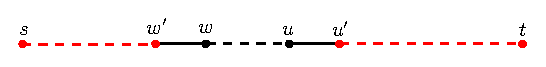
\includegraphics[width=0.6\textwidth]{Fig11}
	  \caption[General component subpaths]{The path through the tree 
	  $\dual{\triang}_T$ connecting nodes $s$ and $t$, which are both
	  part of the connected component $\concomp$. 
	  The path leaves $\concomp$ at $(w',w)$ and re-enters at $(u,u')$.}
	  \label{fig:component_subpaths}
  \end{figure}
  
  The I/O cost of reporting a general connected component includes
  the cost to walk the triangles of $\concomp$, plus the cost
  of walking the boundary of $\concomp$.
  We denote by $h$ the size of the boundary, and summarize our I/O
  costs with the following lemma.

  \begin{lemma}\label{lem:io_eff_ccomp}
  The algorithm $\funccase{DepthFirstTraversal}$ reports a connected 
  component 
  $\concomp$ with $h$ boundary edges using 
  $O\left( \frac{|\concomp|}{\lg{\succblksize}} \right) + O(h \log_{B}{h})$ I/Os.
  \end{lemma} 

  \begin{proof}
  Performing depth-first traversal is equivalent to a walk of 
  length at most $4|\concomp|$, which can be performed in 
  $O\left( \frac{|\concomp|}{\lg{\succblksize}} \right)$ I/Os. 
  We must also account for the length of the paths traversed by calls 
  to $\funccase{ScanBoundary}$. 
  Any triangle in $\concomp$ may be visited at most three times, since 
  it may be adjacent to no more than three different boundary chains. 
  Thus, the total additional length of the walks associated with calls 
  to $\funccase{ScanBoundary}$ is bounded by $3|\concomp|$, which 
  increases the length of the path traversed by a constant factor. 

  We must also account for the number of I/Os required to maintain 
  and query the boundary edge structure $\mathcal{V}$. 
  There are $h$ boundary edges, and in the worst case most of these 
  edges may be access edges. 
  Using a B-tree to store $\mathcal{V}$ 
  supports insertions and queries in $O(\log_B{h})$ time.  
  An access edge is added to $\mathcal{V}$ only once, and is visited at 
  most one additional time. 
  Thus the total cost to maintain and query $\mathcal{V}$ is $O(h \log_B{h})$.  
  \end{proof}

  Finally, we account for the space used to store $\mathcal{V}$. 
  Since our triangulation does not store edges, we must have some
  way of uniquely identifying the edges in $\mathcal{V}$.
  We do so by storing the coordinates of the midpoint of each edge, which
  serves as our search key.
  For $\mathcal{V}$ we use a B-tree, and for each edge store a $\bitsPerPoint$-bit 
  key plus a $\lg{N}$ bit pointer. 
  Thus the space for this structure is $\OhOf{h \cdot(\bitsPerPoint + \lg{N})}$ 
  bits. 
  In theory, the size of this structure could be as large as $\concomp$,
  but in many scenarios it will be significantly smaller.  
  The following theorem summarizes our results 
  for convex and general connected components. 
  The space bound adds the space for $\mathcal{V}$ to the bound from
  Theorem \ref{thm:terrain_traversal}.
  The I/O bounds are obtained from Lemmas \ref{lem:report_convex_component} 
  and \ref{lem:io_eff_ccomp}.

  \begin{theorem}\label{thm:conn_comp}
  A triangulation $T$, with $\bitsPerKey$-bit keys per triangle, may be 
  stored using 
  $N(\bitsPerPoint + \bitsPerKey) + O(N) + o(N(\bitsPerPoint + \bitsPerKey)$ 
  bits such that a 
  connected component $\concomp$ may be reported using 
  $O \left( \frac{|\concomp|}{\lg{B}} \right)$ I/Os if $\concomp$
  is convex.  
  If $\concomp$ may be non-convex or have holes, then the query requires 
  $O\left( \frac{|\concomp|}{\lg{B}}  + h \log_B{h}\right)$ 
  I/Os, plus an additional $\OhOf{h \cdot(\bitsPerPoint + \lg{N})}$ bits of storage, 
  where $h$ is the number of boundary edges of 
  $\concomp$.
  \end{theorem}

  % ----------------------------------------------------------------------
  \subsection{Connected Components Without Additional Storage}
  \label{ssec:no_add_storage}
  % ----------------------------------------------------------------------

  One drawback with our technique for reporting connected components 
  in Section~\ref{ssec:gen_con_comp} is that 
  we must store the search structure $\mathcal{V}$ in order to complete the 
  traversal. 
  In this section, we present a revised version of the algorithm that removes 
  the need for this additional data structure, at the cost of performing 
  additional I/O operations.

  Our technique is based on the algorithm of Bose and 
  Morin~\cite{DBLP:conf/isaac/BoseM00}, for the more general case of subdivision 
  traversal in planar subdivisions. 
  That paper, in turn, is a refinement of the algorithm presented by 
  de~Berg~\etal~\cite{deberg_et_al_1997}. 
  The strategy in both papers is to identify a single entry edge on each face. 
  When an edge is visited while reporting the edges of a face, a check is made 
  to determine if it is the (unique) entry edge for an adjacent face. 
  If the edge proves to be an entry edge, then the adjacent face is entered. 
  The resulting traversal is a depth-first traversal of the faces of the 
  subdivision. 
  In both papers, (\cite{DBLP:conf/isaac/BoseM00} and \cite{deberg_et_al_1997}),
  the subdivision is assumed 
  to be represented as a doubly-connected edge list, or a similar 
  topological structure. 

  Bose and Morin~\cite{DBLP:conf/isaac/BoseM00} select entry edges based 
  on a total order $\preceq_p$ on the edges of the subdivision. 
  The position of each edge, $e$ in $\preceq_p$, is determined based on 
  the edge's key. 
  The key is a 4-tuple of properties that can be calculated locally for 
  each edge, based on the edge's geometry. 
  As with our previous entry edge seletion rule, the keys are calculated 
  with repect to a known point interior to the start triangle.
  To determine if an edge is the entry point of a face, the following 
  \emph{both-ways} search is performed.
  Starting at edge $e$, the face is scanned in both directions 
  until either (a) an edge $e'$ is encountered with 
  a lower key than $e$ in $\preceq_p$, or (b) the scans meet without 
  having found any such edge.  
  In case (b), the edge $e$ is then selected as the entry edge for 
  the face.

  The main result of Bose and Morin is that for a subdivision 
  with $N$ vertices, all faces (including edges and vertices) can be 
  reported in $\OhOf{N \log{N}}$ steps. 
  Their approach can also be applied to reporting a connected 
  component of the subdivision in $\OhOf{h \log{h}}$ time, where the 
  $h$ is the number of vertices in the component.  

  In this paper all faces are triangles, thus to find the entry edge
  at the triangle level is a constant-time operation using any
  selection technique.
  Where the 'search both ways' technique proves useful in our setting 
  is in dealing with the boundary of the component. 
  A hole may consist of 
  one or many faces (triangles), but we treat a hole as if it were a 
  single face.
  For each hole, we want to identify a unique entry edge from among
  the access edges on its boundary.
  Since edges are not explicity stored in our construction, walking
  the boundary involves walking the set of triangles that touch the boundary. 
  This includes all triangles in $\concomp$ that:
  
  \begin{enumerate}
  \item have an edge on the boundary, or
  \item have an adjacent vertex, $p \in P$, that lies on the boundary.
  \end{enumerate}
  
  Let $h'$ denote the number of triangles touching the boundary of
  $\concomp$. 
  This includes both holes in $\concomp$ and its outer boundary.
  A triangle can be adjacent to the boundary at no more than three 
  points (or edges), therefore $h' = \OhOf{|\concomp|}$. 
  
  Assume $H$ is some hole in our component. 
  In order to apply the analysis of Bose and Morin directly to our results, 
  we conceptually add zero length
  \emph{pseudo-edges} to $H$ at any point on the boundary of $H$ that 
  is adjacent to a triangle $t$ which touches $H$ at a point, but which 
  does not share an edge with $H$ (see Fig. \ref{fig:pseudo-face} ). 
  With respect to the key values in $\preceq_p$, we set the value of 
  a key for a pseudo-edge to $\infty$. 
  Since the entry edge in any hole is the edge of minimum key value, 
  no pseudo-edge will ever be selected. 
  Given this definition of a pseudo-edge, the value $h'$ can also 
  be considered the sum of real and pseudo-edges over all holes 
  and the exterior boundary of the component $\concomp$.

  \begin{figure}[th]
	  \centering
		  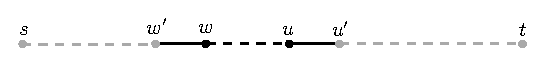
\includegraphics[width=0.8\textwidth]{Fig12}
	  \caption[Psuedo-edges in region boundaries]{The figure on the left 
    shows a portion of a component (grey) with a hole (white). 
	  The dashed box indicates the detailed area shown in the figure on the
	  right. 
	  The right-hand figure shows conceptually how additional edges are 
	  added to the hole boundary, corresponding to triangles in the component.
	  At the point marked $a$, a single pseudo-edge is added as there is 
	  only one non-edge adjacent triangle adjacent to this point. 
	  The point $b$ has two non-edge adjacent triangles, therefore two pseudo-edges 
	  $b$ and $b'$ are added to the hole boundary. }
	  \label{fig:pseudo-face}
  \end{figure}

  The following lemma summarizes results for Bose and Morin that can now be 
  applied directly to our setting.

  \begin{lemma}\label{lem:bose_morin_time}
  For a connected component $\concomp$ requiring $h'$ triangles to be visited 
  in order to walk the boundary of all holes plus the exterior boundary of 
  $\concomp$, the both-ways search technique can find entry edges for all 
  holes (and the perimeter) in at most $\OhOf{h' \log{h'}}$ steps, 
  or $\OhOf{h' \log_{\succblksize}{h'}}$ I/Os. 
  \end{lemma}

  \begin{proof}
  Theorem 1 in Bose and Morin \cite{DBLP:conf/isaac/BoseM00} states that 
  a planar subdivision of faces with $n$ vertices can be traversed in 
  $\OhOf{n \log{n}}$ time. 
  By adding zero-length pseudo-edges, we effectively make 
  the set of holes and the exterior boundary equivalent to faces with 
  a total of $h'$ edges. 
  Thus, using the both-ways search, we can locate entry edges with 
  $\OhOf{h' \log{h'}}$ steps. 
  Since we can travel $\OhOf{\log{\succblksize}}$ steps during such 
  searches before incurring an I/O, we can perform all such searches in 
  $\OhOf{h' \log_{\succblksize}{h'}}$ I/Os.
  \end{proof}

  Applying the both-ways search technique presented above requires only 
  minor modifications to our algorithms. 
  In the $DepthFirstTraversal$ algorithm (Fig. 
  \ref{fig:traverse_graph_algorithm}) at line 7 rather than check 
  if $e \in \mathcal{V}$, we perform the both-ways search to determine 
  if $e$ is the unique entry edge. 
  If this is true, we then perform $ScanBoundary$ starting with $e$. 
  The only alteration to the $ScanBoundary$ algorithm 
  (Fig. \ref{fig:scanhandrail_alg}) is that we can omit steps 3 
  through 9, since following the both-ways search we know that $e$ 
  is the  unique entry edge for the boundary or hole.  

  To summarize we have the following theorem.

  \begin{theorem}\label{thm:conn_comp_without_add_storage}
  A triangulation $\triang$, with $\bitsPerKey$-bit keys per triangle, 
  may be stored using $N\bitsPerKey + O(N) + o(N\bitsPerKey)$ bits such 
  that a connected component $\concomp$ may be reported using 
  $\BigOh{\frac{|\concomp|}{\lg{B}} + h' \log_B{h'}}$ I/Os, where 
  $h'$ is the total number of triangles that touch all holes in, 
  plus the boundary of, $\concomp$.
  \end{theorem}
